% id: 0421
% book: RPM 중3-2 수학 · 04 원주각
% section: 유형 05 원주각의 성질과 삼각비의 값
% figure: crop:fig-0421.png
% answer: ①
% answer_source: 답지
% variant_level: 0 (원본 전사)
% 이 파일은 build.mjs 가 items.json 에서 만든다. 고칠 때는 items.json 을 고친다.
\noindent\begin{minipage}[t]{0.58\linewidth}\vspace{0pt}\raggedright 오른쪽 그림과 같이 $\seg{AB}$를 지름으로 하는 원~$\pt{O}$에서 $\angle\pt{CAB}=30^\circ$일 때, $\triangle\pt{ABC}$의 둘레의 길이는?\end{minipage}\hfill\begin{minipage}[t]{0.4\linewidth}\vspace{0pt}\centering \setlength{\dmfigw}{81.4pt}\ifdim\dmfigw>\linewidth\setlength{\dmfigw}{\linewidth}\fi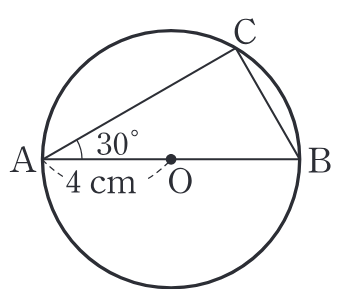
\includegraphics[width=\dmfigw]{figures/fig-0421.png}\end{minipage}\par
\begin{choicesv}{$(12+4\sqrt{3})\mkern3mu \mathrm{cm}$}{$(12+6\sqrt{3})\mkern3mu \mathrm{cm}$}{$20\mkern3mu \mathrm{cm}$}{$(16+4\sqrt{3})\mkern3mu \mathrm{cm}$}{$(16+6\sqrt{3})\mkern3mu \mathrm{cm}$}\end{choicesv}
